\chapter{Analýza}
\label{chapter:analyza}
Hlavním cílem teto bakalářské práce je implementovat návrh backendu podle návrhu a fragmentu implementace, které byly udělány v rámci předmětů BI-SP1 a BI-SP2 bakalářského studia vyučovaných na FIT ČVUT v akademickém roce 2018/2019 a 2019/2020. Tato kapitola se zabývá analýzou výsledků zmíněných předmětu. Autor práce je zároveň i absolventem těchto předmětů, kde pracoval v týmu na analýze požadavku zákazníka a pak pracoval jako backend vývojář a vedoucí backendového týmu.

Pro jasné zajištěni verze aplikace, která bude předmětem analýzy teto kapitoly, uvádím datům ukončení práce na projektu v rámci předmětu BI-SP2 - 25. února 2020. Také, pro možnost pohodlně vyhledat konkretní verze na GitLabu (\url{https://gitlab.fit.cvut.cz/rozvody/be-springboot}), uvádím poslední \textit{commit}\footnote{proces při kterém se uloží všechny udělané v rámci systému řízení verzí změny a zařadí se do historie změn} udělaný přes Git\footnote{ distribuovaný systém řízení verzí} v rámci tohoto předmětu: 
\begin{quote}
    \enquote{252b0288dbfe9942446b78fd452c0edce810a370}
\end{quote}

% Tato kapitola se zabývá popisem současného stavu aplikace, který je výsledkem zmíněných předmětů.

% Hlavním cílem teto bakalářské práce je implementovat návrh backendu podle návrhu a fragmentu implementace, které byly rozpracovány v rámci předmětů BI-SP1 BI-SP2 bakalářského studia vyučovaných na FIT ČVUT. Dalším cílem teto práci je navrhnou vhodné úpravy za účelem dosažení kvalitnějšího výsledku a splnění požadavku frontedové častí aplikace. Autor teto práci absolvoval zmíněné předměty, proto pro zajištění rozdilu v 

\section{Analýza současného návrhu} \label{analyza:analyza navrhu}
    
    \subsection{Předmět BI-SP1}\label{analyza:navrh:sp1}
    V rámci předměty BI-SP1 pracovalo sedm lidí včetně autora teto práci. Tým měl za úkol analýz požadavku zákazníka a návrh implementaci aplikace. Aplikace se skládá ze dvou částí. Serverového backendu, který je předmětem teto bakalářské práci a frontendové častí aplikace, kterou současně v rámci bakalářské prací implementuje kolega - Martin Beran. Frontendová část aplikace je Android aplikací. Backendová část je serverovým backendém, který má poskytovat REST\footnote{Representational State Transfer} API pro Android aplikaci.
    
    Během semestru tým provedl kompletní analýzu požadavku zákazníka. Především, tým navrhl scénáře použiti aplikace:
    \begin{itemize}
	   \item Přihlašování/Registrace;
	   \item Přihlašování/Registrace do rodiny;
	   \item Role v aplikace a jejich vytváření;
	   \item Nastavení pečovatelský dnů;
	   \item Kalendář;
	   \item Kniha potřeb dítěte;
	   \item Uchování účtenek;
	   \item Správa alimentů.
	\end{itemize}
    Potom byly navrženy Diagram užití\footnote{popisuje chování systému z vnějšího pohledu} a Diagram aktivit\footnote{zobrazuje jak objekty spolupracují}, podle kterých byly navrženy Wireframy\footnote{grafickém zobrazením hlavních prvků frontendové častí aplikace} a Doménový model\footnote{náčrt základních entit systému a vztahů mezi nimi}. 
    
    \subsection{Předmět BI-SP2}\label{analyza:navrh:sp2}
        Cílem předmětu BI-SP2 byla implementace návrhu předmětu BI-SP2. Autor teto práce pracoval v backendovém týmu a zároveň vystupoval v roli vedoucího backendového týmu.
        
        Pro vývoj backendové častí aplikace byl zvolen jazyk Kotlin, zmíněný v sekci \ref{resere:kotlin}, a framework Spring, zmíněný v sekci \ref{resere:j2ee}. Jako {buildovací system}\footnote{nástroj pro automatizaci sestavování programu} byl zvoleny nástroj Gradle. Podrobnnějí výsledky předmětu BI-SP2 probrány v sekce \ref{analyza:soucasnaImplementace}.
        
    
    \subsection{Doménový model}\label{analyza:navrh:DomainModel}
        Hlavním zdrojem informace o výsledném návrhu serveru je Doménový model. Kompletní Doménový model se nachází v příloze \ref{dodatek:DomainModel}. Zelenou barvou jsou označeny třídy, které už jsou implementovány. žlutou barvou jsou označeny třídy, které ještě nejsou implementovány. Také, jsou třídy označeny zároveň žlutou a zelenou barvou, což znamená, že třída je implementována jenom částečně. Taková situace se mohla nastat v případe, že implementace vyžadovala implementace jiné třídy, která ještě neexistovala. Tento Doménový model má určité nedostatky podle požadavku frontedové části aplikace. Jako příklad takových nedostatku je možné uvést zbytečně komplikovaný návrh entity \textit{Interval} (viz. obrázek \ref{image:Interval1}), který byl úplně předělán.

    \subsection{Registrace a přihlášeni do rodiny}
        Aplikace je navržena tak, že první uživatel, který má vytvořit svůj účet je jeden z rodičů. Pro registraci člověk potřebuje řadu povinných údajů:
        \begin{itemize}
	        \item \textit{name} - zvolené jméno se stává jeho implicitním jménem v systému
	        \item \textit{surname} - zvolené příjmení se stává jeho implicitním příjmením v systému
	        \item \textit{email} - zvolený email je identifikátorem uživatele v rámci systému
	        \item \textit{password} - heslo pro autorizaci v systému
        \end{itemize}
        Na základe těchto údajů se vytváří unikátní uživatel v rámci systému. V tomto stavu člověk není přihlášeny do žádné rodiny a nemá žádnou roli. Podrobněji role budou popsané v sekci \ref{analyza:bezpecnost:role}. \textit{User} také může mít implicitní obrázek profilu (viz. obrázek \ref{image:User-Image1}).
        \begin{figure}\centering
	        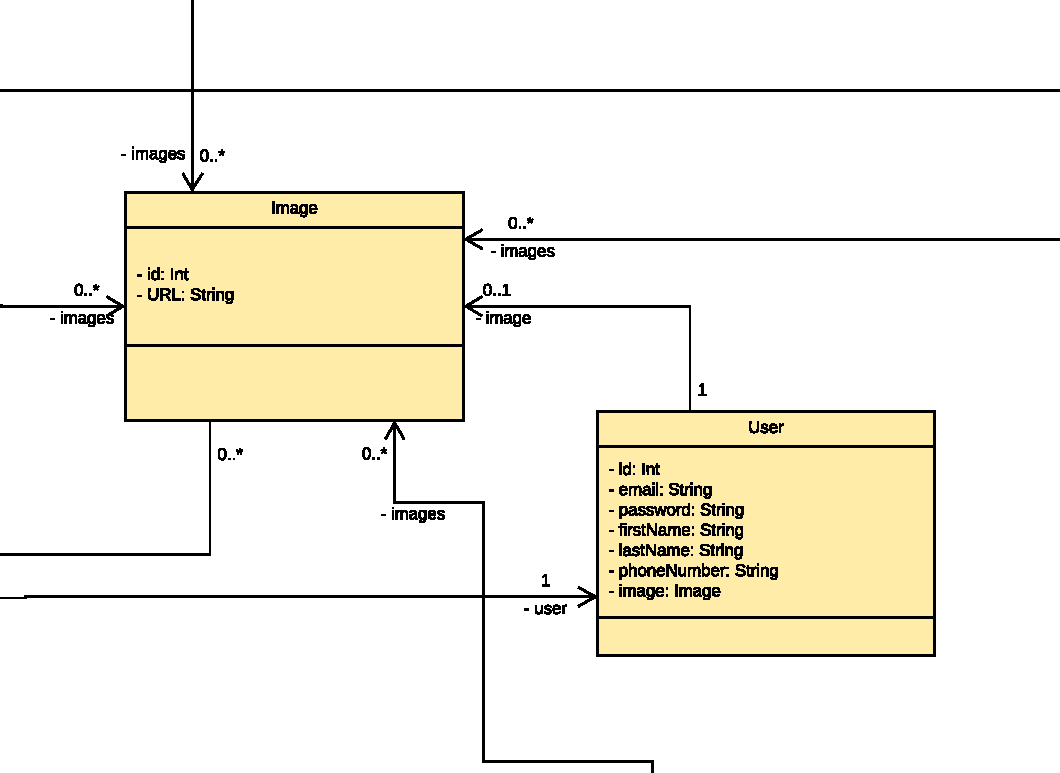
\includegraphics[width=0.5\textwidth]{pdfs/User-Image1}
	        \caption[Návrh User-Image]{Vztah mezi třídami \textit{User} a \textit{Image} podle Doménového modelu z předmětu BI-SP2}\label{image:User-Image1}
        \end{figure}
        
        Potom uživatel má možnost vytvořit rodinu nebo přihlásit se do již existující rodiny. Pro vytvoření nové rodiny, uživatel potřebuje zadat jméno rodiny a přidat členy rodiny. Autor teto rodiny automaticky se stává jedním s rodičů teto rodiny. jinou možností je přihlásit se do rodiny, která již existuje. Podmínkou k tomu je existování pozvání do některé existující rodiny. V takovém případě uživatel už nemá možnost zvolit role v rámci rodiny. Role má být nastavena uživatelem, který vytvořil toto pozvání.

    \subsection{Kalendář}    
        Kalendář je hlavním zdrojem informaci pro celou rodinu, který společný pro všechny uživatele. Na něm jsou zobrazené zvýrazněné různými barvami pečovatelské dny obou rodičů a důležité události, které mohou být jednorázové nebo pravidelné. 
        
        Kromě dlouhodobých nastavení pečovatelských dnu, kalendář může zobrazovat i jednorázové změny, které mohou vidět všechny členy rodiny. Takový postup pomáhá rodině eliminovat situace, kdy několik členu rodiny najednou myslí, že je v konkretní den dítě v jejích péči nebo několik členu rodiny najednou říkají, že není to jejích den.  
    \subsection{Alimenty}    
        Aplikace řeší i finanční problémy. Hlavním problémem jsou alimenty, které má pravidelně uhrazovat jeden z rodičů. Tento proces byl rozdělen do dvou častí. První častí je dlouhodobé nastávení alimentů (viz. obrázek \ref{image:AlimonySettings1}) . Druhou častí jsou samotné alimenty (viz. obrázek \ref{image:Alimony1}), které se generuje na základě dlouhodobých nastavení. Jedna rodina může mít zároveň několik nastavení v případě, že jedna rodina má několik dětí nebo chce rozdělit alimenty do logických částí.
        \begin{figure}\centering
	        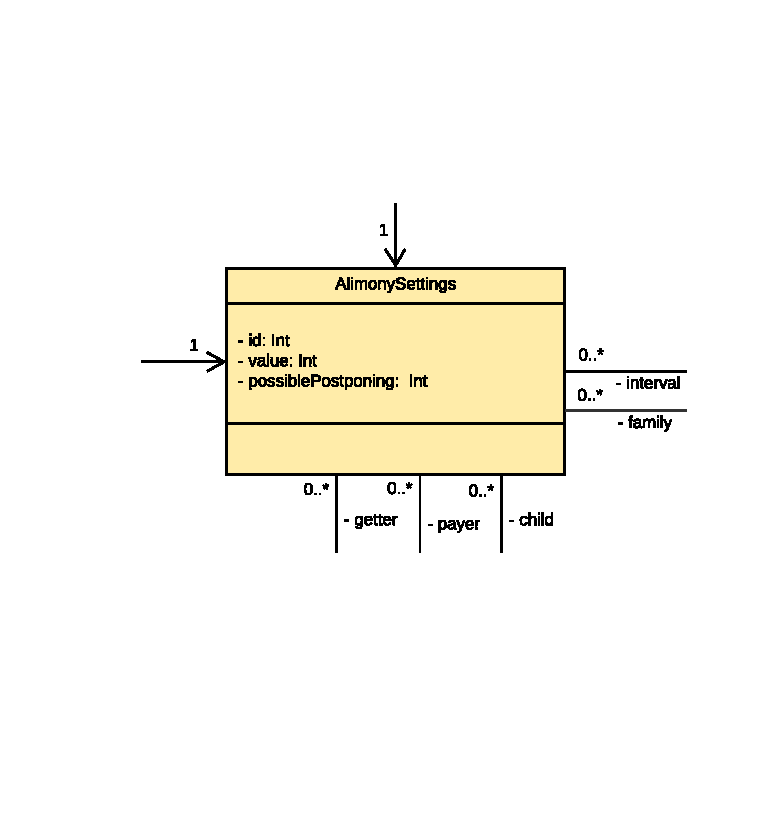
\includegraphics[width=0.5\textwidth]{pdfs/AlimonySettings1}
	        \caption[Návrh AlimonySettings]{Návrh třídy \textit{AlimonySettings} podle Doménového modelu z předmětu BI-SP2}\label{image:AlimonySettings1}
        \end{figure}
        \begin{figure}\centering
	        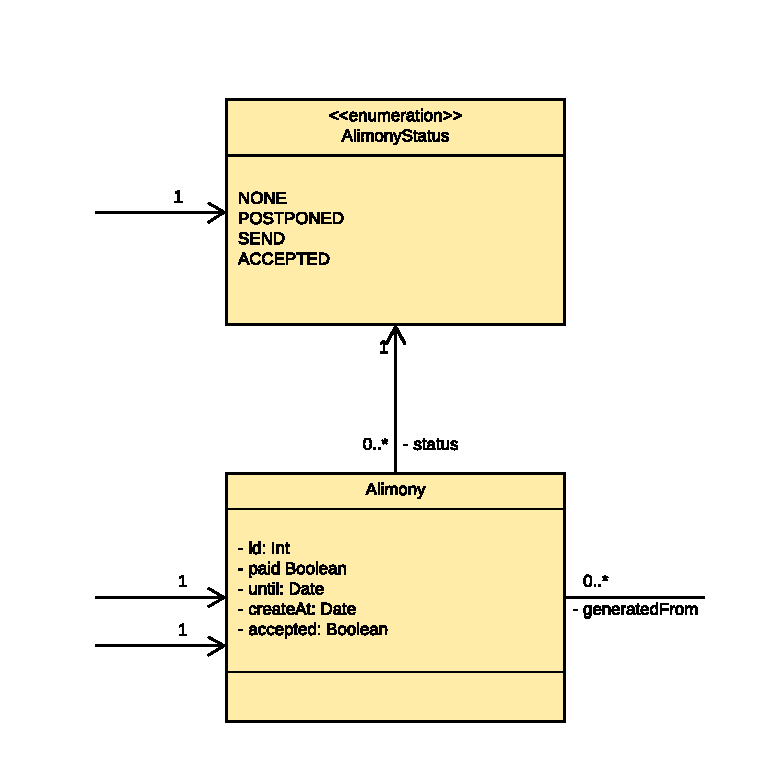
\includegraphics[width=0.5\textwidth]{pdfs/Alimony1}
	        \caption[Návrh Alimony]{Návrh třídy \textit{Alimony} podle Doménového modelu z předmětu BI-SP2}\label{image:Alimony1}
        \end{figure}
    \subsection{Kniha potřeb dítěte}
    
        Jedním s populárních problému, které vznikají v procesu rozvodu, je nakupování příliš drahých věci o kterých nevědí ostatní členy rodiny. Jako příklad je možné uvést nakupování bot pro dítěte. Jeden s rodičů může chtít \enquote{koupit lásku dítěte} a koupit několikrát dražší boty než dítěte opravdu potřebuje. Kniha potřeb dítěte (viz. obrázek \ref{image:Need1}) je zaměřena na překonání takových situací.
        \begin{figure}\centering
	        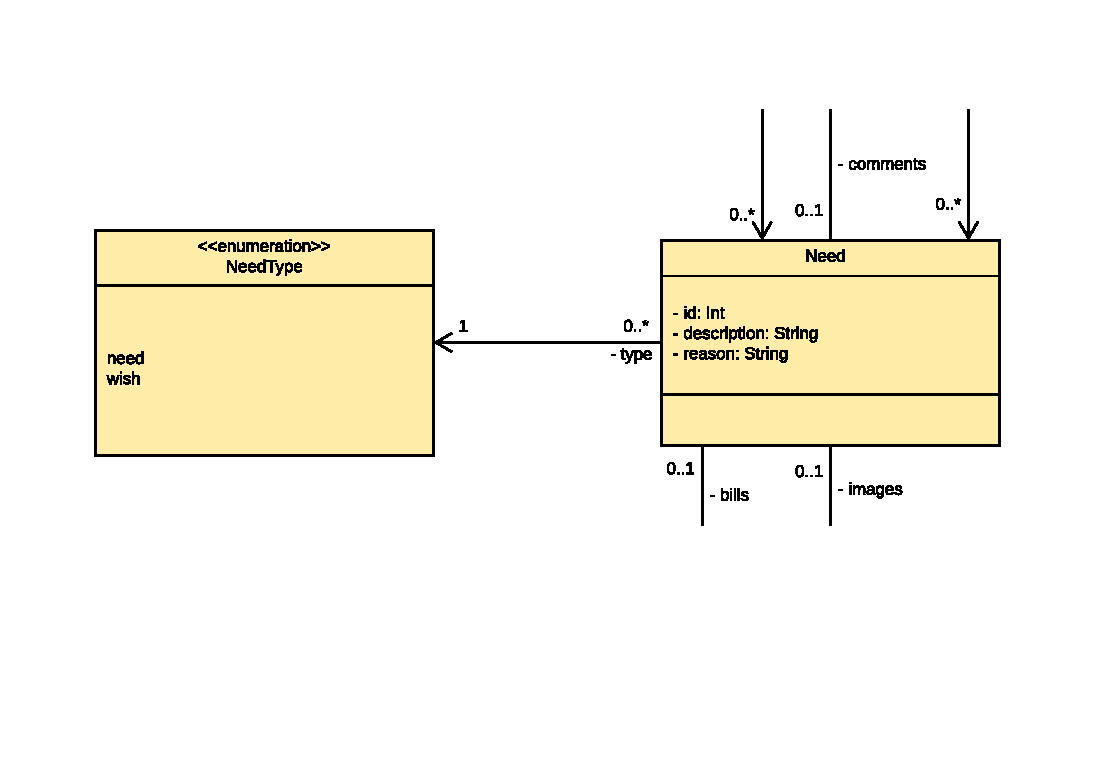
\includegraphics[width=0.5\textwidth]{pdfs/Need1}
	        \caption[Návrh Need]{Návrh třídy \textit{Need} podle Doménového modelu z předmětu BI-SP2}\label{image:Need1}
        \end{figure}
        
        Potřeba může být typu \textit{need} a \textit{wish}. Podle současného návrhu je rozdíl mezi typy pouze pro informační účely. Každé instance \textit{Need} patři instance \textit{NeedPermission} (viz. obrázek \ref{image:NeedPermissions1}), která definuje přístupová práva pro jednotlivé členy rodiny. V případě, že uživatel nemá žádné z přístupových práv, potřeba se nevyskytuje v jeho seznamu potřeb dítěte. Toto pravidlo se netýká jenom rodičů, která mají přistup ke všem potřebam automaticky. 
        \begin{figure}\centering
	        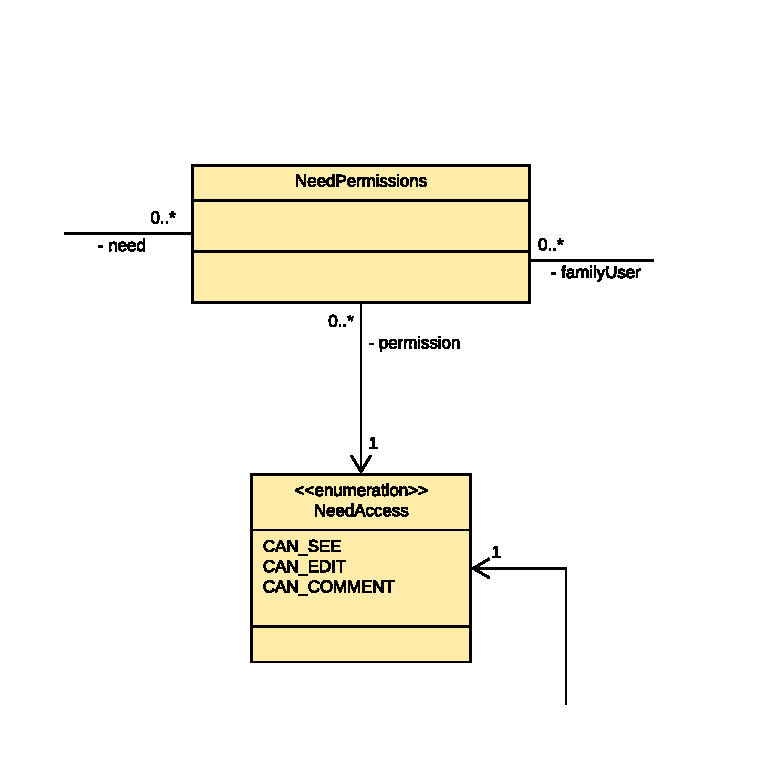
\includegraphics[width=0.5\textwidth]{pdfs/NeedPermissions1}
	        \caption[Návrh NeedPermissions]{Návrh třídy \textit{NeedPermissions} podle Doménového modelu z předmětu BI-SP2}\label{image:NeedPermissions1}
        \end{figure}
       
       Potřeba má v sobě následující informace:
        \begin{itemize}
            \item \textit{description} - popis potřeby
            \item \textit{reason} - příčina proč dítě tohle potřebuje
            \item \textit{images} - obrázky věcí, kterou dítě potřebuje
            \item \textit{bills} - účtenky v případě, že někdo z rodičů splnil potřebu
            \item \textit{comments} - komentáře členu rodiny včetně dítěte
        \end{itemize}
     
\section{Analýza současné implementace}\label{analyza:soucasnaImplementace}
    \begin{figure}\centering
	   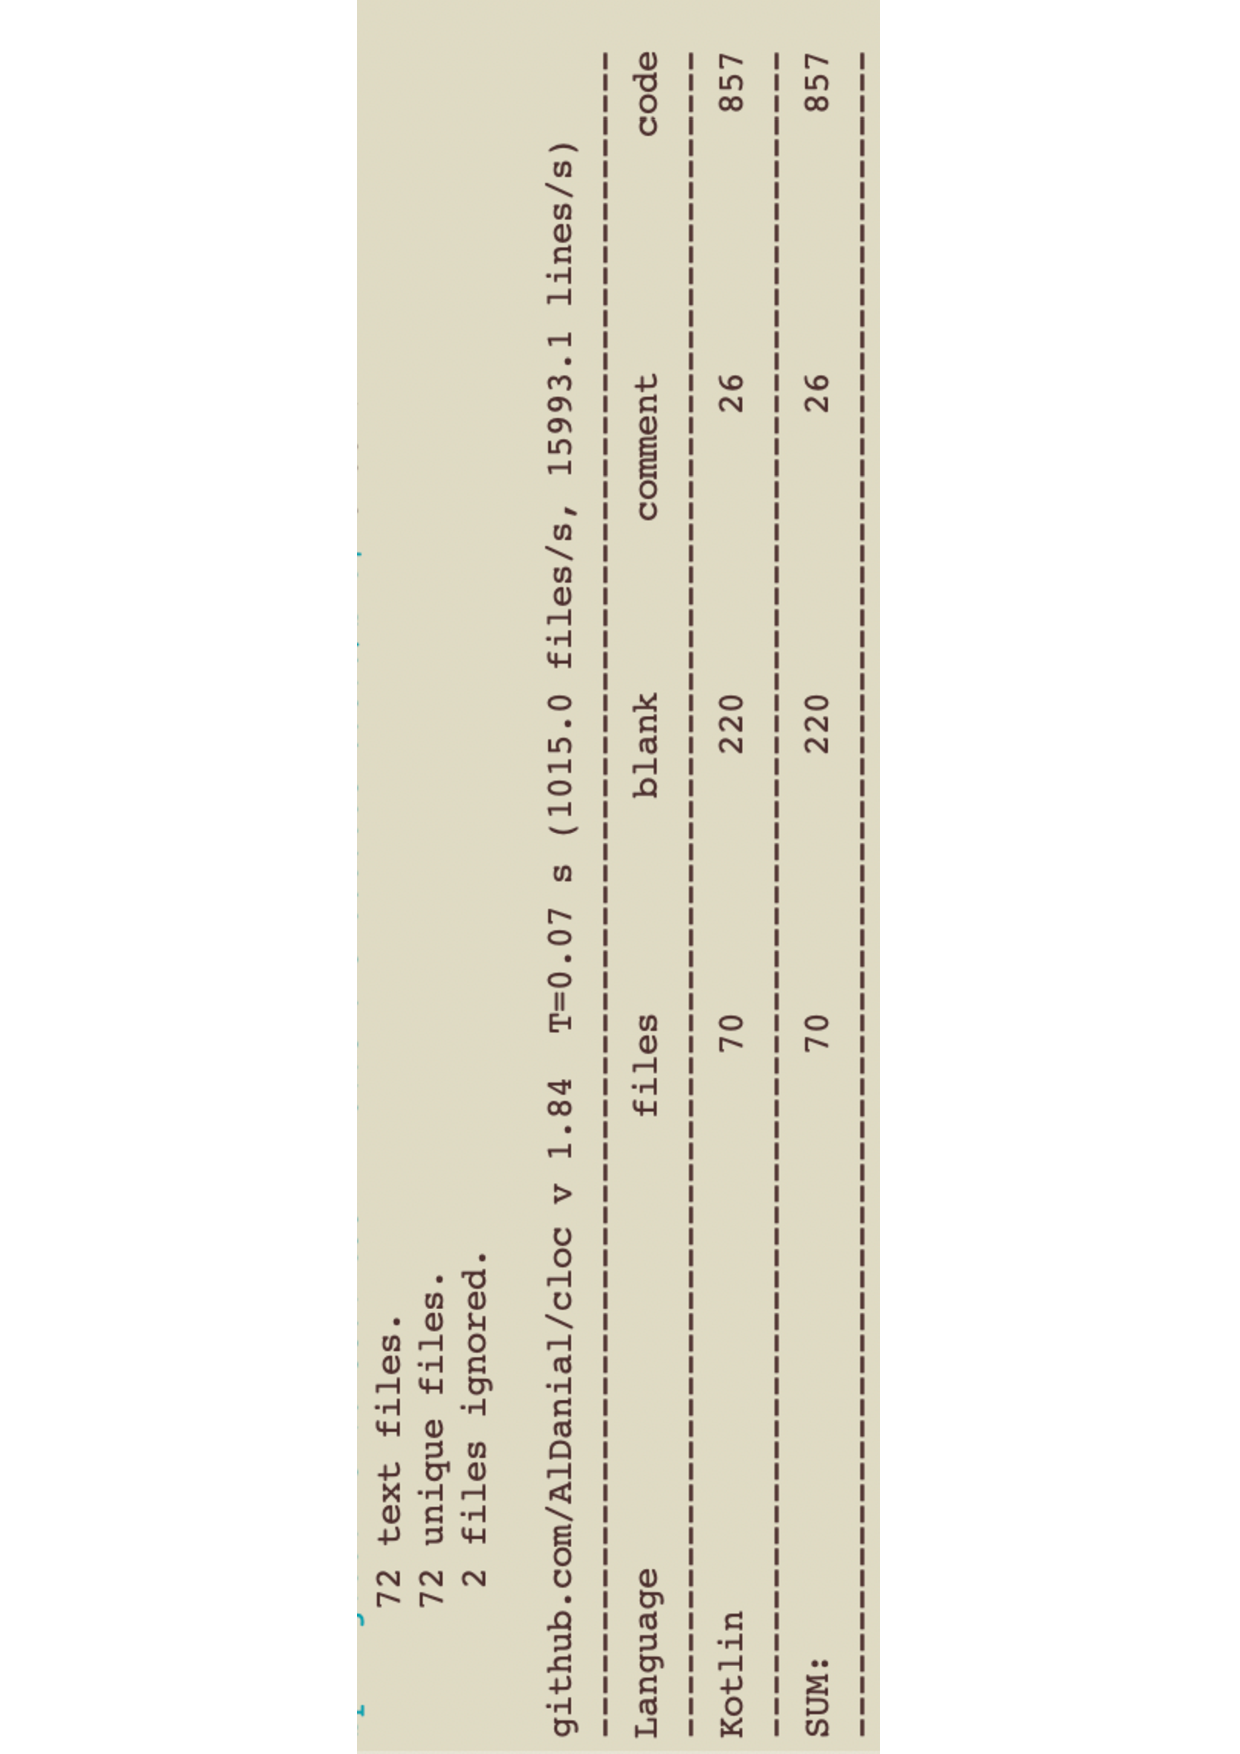
\includegraphics[angle=-90, width=0.7\textwidth]{pdfs/Cloc1}
	   \caption[Počet řádků kódu před začátkem práce]{Počet řádků kódu před začátkem práce}\label{image:cloc1}
    \end{figure}
     V teto sekci bude stručně popsán soćasný stav implementace. Současná implementace obsahuje 69 souborů a 845 řádek kódů (viz. obrázek \ref{image:cloc1}), které byly vytvořeny a napsány členy týmu. Za účelem zvětšení přesnosti analýzy byl zvolen nástroj pro analýzu počtu řádek kódu - CLOC (viz. sekci \ref{reserse:cloc}). Implementace částečné pokrývá Doménový model zmíněný v sekci. \ref{analyza:navrh:DomainModel}.
        
    \subsection{Implementované třídy}
        Seznam implementovaných entit:
        \begin{itemize}
            \item \textit{AlimonyStatus}
            \item \textit{Bill}
            \item \textit{CalendarEvent}
            \item \textit{OneTimeEvent}
            \item \textit{Comment}
            \item \textit{FamilyMember} - částečně
            \item \textit{History}
            \item \textit{IntervalType}
            \item \textit{NWeekInterval}
            \item \textit{WeekInterval}
            \item \textit{NeedAccess}
            \item \textit{NeedType}
            \item \textit{NeedType}
            \item \textit{AbstractPermissions}
            \item \textit{Permissions}
            \item \textit{RequestStatus}
            \item \textit{User}
        \end{itemize}
        
        Byl přidán \textit{controller}\footnote{vrstva controlleru zajišťuje REST API komunikaci, překládá výjimky na HTTP kóda zajišťuje omezení pro jednotlivých uživatelů} pro testování, zda aplikace běží, který je namapován\footnote{přidání konkrétnímu controlleru adresy pomocí anotací frameworku Spring, která se zadává jako URI při odesílaní požadavků na Server} na cestu \enquote{/}. Také, byla přidaná třída, která obsahuje nápovědy pro ostatní \textit{controllery} ohledně zachycování chyb. Tato třída byla zavedena za účelem poskytování uživateli jenom korektně formátovanou informaci  a filtrování zbytečné informace pro koncového uživatele (viz. tabulka \ref{tab:excpetion-handler1}). 
        \begin{table}\centering
	    \caption[Exception handler]{Ukázka \textit{Exception handler} podle návrhu BI-SP2}\label{tab:excpetion-handler1}
	    \begin{tabular}{|l|c|c|c|}\hline
		  Typ chyby		& HTTP status		& zprava	& URL	\tabularnewline \hline \hline
		  \textit{Illegal Access}	& 401	& původní zprava chyby		& původní cesta     \tabularnewline \hline
		  \textit{Illegal Argument}	& 400	& původní zprava chyby		& původní cesta     \tabularnewline \hline
		  \textit{Null Pointer}	& 500	& původní zprava chyby		& původní cesta     \tabularnewline \hline
		  \textit{No Such Element}	& 404	& nic		& nic     \tabularnewline \hline
	    \end{tabular}
        \end{table}
    
    \subsection{Dokumentace API}
        Bylo provedeno nastavení frameworku Swagger pro dokumentace API (viz. obrázek \ref{code:swagger-configuration}). Podrobněji framework Swagger byl popsán v sekci \ref{resere:dokumentace}.
        \begin{figure}
        \begin{minted}{java}
@Configuration
@EnableSwagger2
class SwaggerConfig {
@Bean
fun api(): Docket {
    return Docket(DocumentationType.SWAGGER_2)
        .select()
        .apis(RequestHandlerSelectors.any())
        .paths(PathSelectors.any())
        .build()
    }
}
        \end{minted}
        \caption{Ukázka nastavení frameworku Swagger}\label{code:swagger-configuration}
        \end{figure}
    
    \subsection{Profily}\label{analyza:soucasnaImplementace:profily}
    %spring profiles: https://docs.spring.io/spring-boot/docs/current/reference/html/spring-boot-features.html#boot-features-profiles
    %applicatioon peoperties: https://docs.spring.io/spring-boot/docs/current/reference/html/spring-boot-features.html#boot-features-external-config-application-property-files
        Framework Spring poskytuje možnost rozdělit implementaci do logických bloků, které budou existovat jenom v konkrétních profilech\cite{spring-profile}. Implicitně všechny komponenty nezávisle na aktuálních profilech. Pro zavedení profilů pro konkretní komponentu je potřeba ji označit anotací \textit{Profile}. V závorkách vedle anotací je potřeba přidat seznam profilu, ve kterých tato komponenta bude existovat. Konfigurace aktuálně zapnutých profilů se provádí pomocí souboru \textit{application.properties}, který definuje proměnné pro prostředí aplikace. Soubor se nachází ve slo+zce s cestou \enquote{be-springboot/src/main/resources}.
    
        Každý profil také může obsahovat vlastní konfigurační soubor, který definuje všechny nutné proměnné. Soubor má byt zadán ve formátu \textit{application-\{profile\}.properties}, kde \textit{profile} je názvem profilu kterému patří tento soubor. Současný návrh aplikace obsahuje dva konfiguračních souboru.
    
        První konfigurační soubor obsahuje implicitní proměnné pro prostředí aplikace. Aktuálně soubor má jenom definici aktuálního profilu aplikace. 
    
        Druhý konfigurační soubor patří profilu \textit{development}. Tento profil je určen pro pohodlný proces vývoje aplikace. Soubor obsahuje konfiguraci databáze a konfiguraci žurnálu aplikace. Podrobněji použita databáze pude popsána v sekci \ref{analyza:soucasnaImplementace:databaze}.
        
    \subsection{Databáze}\label{analyza:soucasnaImplementace:databaze}
        Pro proce vývoje byla zvolena relační databáze H2. Zvolená databáze umožňuje vytvářet tabulky při každém zapuštěni aplikace přímo v pamětí aplikace. Podrobněji tato databáze a její princip fungování byly popsány v sekci \ref{resere:databaze} .
    
\section{Analýza požadavku frontendu na změny}\label{analyza:pozadavky-frontendu}
    V rámci předmětu BI-SP2 současně s implementací backendové častí aplikace, probíhala implementace forntendové častí aplikace - Android aplikace. Během vývoje frotnendové častí aplikace byly zjištěny nedostatky, které zbytečně komplikují implementaci, jak backendu, tak i frontendu.
    
    \subsection{Interval}
        Prvním takovým příkladem je návrh intervalu \ref{image:Interval1}, které jsou široce využívány v projektu. Návrh řešení tohoto problému bude popsán v sekci \ref{navrh:upravy}. tady bude popsán jenom problém samotný. Entita \textit{Interval} reprezentuje časové rozmezí pro pečovatelské dny, opakované události, nastavení alimentů a navazující na ně požadavky na změny a historické záznamy.
            
        Jádro problému je v tom, že entita je navržena pomoci generalizace, neboli dědičnosti z hlediska implementace. Takový návrh dává možnost vytvořit konkretní typ intervalu pomocí zvolení odpovídající třídy, ale na druhou stranu působí komplikace při implementace a nepokrývá všechny možné případy potřebných intervalu. Například, není možné sestavit interval, který se bude opakovat každý poslední den měsíce. Pokud by jsme chtěli se držet se aktuální implementaci a zároveň pokryt všechny možné případy, ztratili bychom přehlednost zvolení správné třídy při vytváření instance \textit{Intervalu}.
            
        Dalším problémem \textit{Intervalu} je provázanost s pečovatelskými dny. Podle návrhu frontendové častí se bylo zjištěno, že pečovatelské dny nepotřebují komplikované nastavení a zároveň bych potřebovali mít odkazy na konkretního rodiče, který je zodpovědný za dítěte v tento den nebo časový úsek.
    
    \subsection{Alimenty}
        Druhou úpravou návrhu backendu, kterou potřebuje frontend, se tyká entity \textit{ALimony}.
        Tato entita reprezentuje alimenty, které jeden rodič má posílat druhému rodiče. Jedna instance se odpovídá alimentům za jeden měsíc. Současný návrh popisuje návrh entity a její navázanost na entitu \textit{AlimonySettings}(viz. obrázek \ref{image:aliomny-draft1}), která definuje dlouhodobou konfiguraci, na základě které se vytváří jednotlivé instance alimentů. Nastavení alimentů se platí v rámci jedné rodiny. V případě potřeby, rodiče mají možnost rozdělit alimenty do několika nastavění. 
        
        Hlavní problém je v tom, že instance alimentů by se měly vytvářet nezávisle na frontendové části aplikace. Podrobně návrh řešení problému bude popsán v sekci \ref{navrh:upravy:alimenty}.
        
        Dodatečným požadavkem frontendového týmu se týká entity \textit{Alimony} samotné. Za účelem zjednoduďení návrhu frontendové části je potřeba přidat závislost na entitu \textit{Family}. % V takovém pŕípade aplikace může ihned po nalazení novych alimentu rict uZivateli ktere rodine patri tyto alimenty.
        \begin{figure}\centering
	        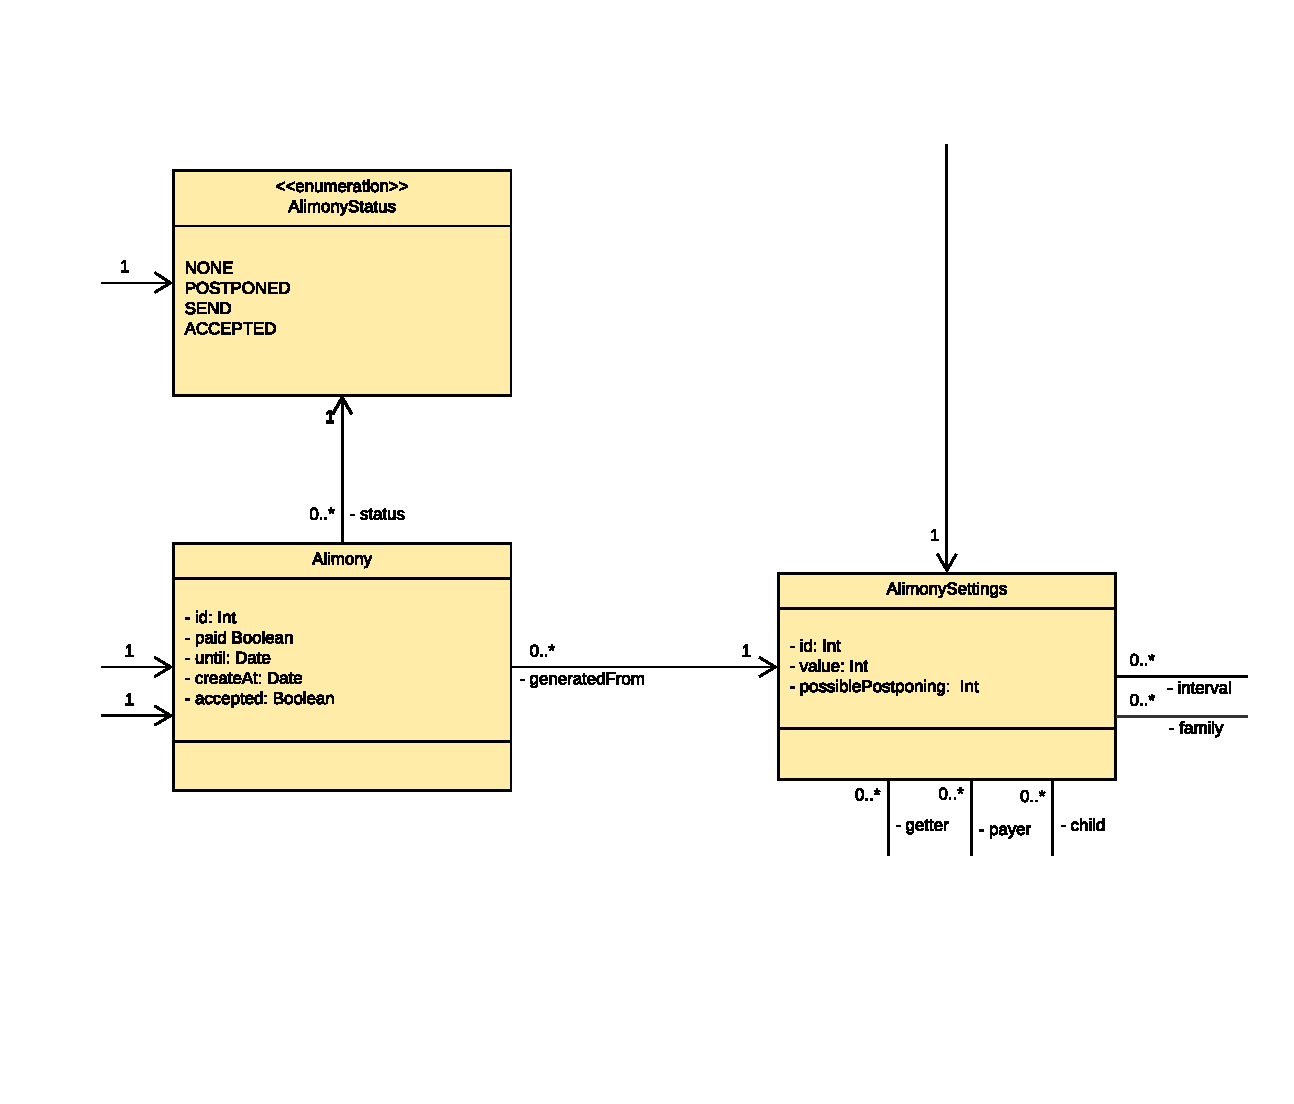
\includegraphics[width=0.5\textwidth]{pdfs/AlimonyDraft1}
	        \caption[Návrh \textit{Alimony} a \textit{AlimonySettings}]{Návrh entit \textit{Alimony} a \textit{AlimonySettings} podle Doménového modelu z předmětu BI-SP2}\label{image:aliomny-draft1}
        \end{figure}
        
        \subsection{Pečovatelské dny}\label{analyza:pozadavky:caredays}
            Než se zanořit do podrobného popisu problému, je potřeba popsat účel teto entity a její využiti backendém a frontendém. Tato entita reprezentuje jednorázový interval nebo opakující interval pečovatelských jednoho z rodičů nebo libovolného jiného člena rodiny. Každý člen rodinu má vlastní barvou, která se využívá pro označování pečovatelských dnů v kalendáři. Tato entita se používá za dvěma účely. První a nejdůležitější účel je nastavení pečovatelských dnů pro rodiče. Nastavení musí pokrývat všechny dny kalendáře. Dítě by nemělo mít ve svém kalendáři den, který není označen žádnou barvou zároveň by neměly vznikat konflikty. Druhým účelem jsou jednorázové změny pečovatelských dnů. Tyto změny jsou vyžadovány pro případy, kdy dlouhodobé nastavení kalendáře neplatí. Příkladem může být výlet dítěte k babičce a dědečkovi. Během tohoto časového intervalu rodiče nejsou zodpovědné za dítěte, proto je potřeba uvést jednorázovou změny do kalendáře, která zaznamená tuto situaci 
            
            \begin{figure}\centering
	            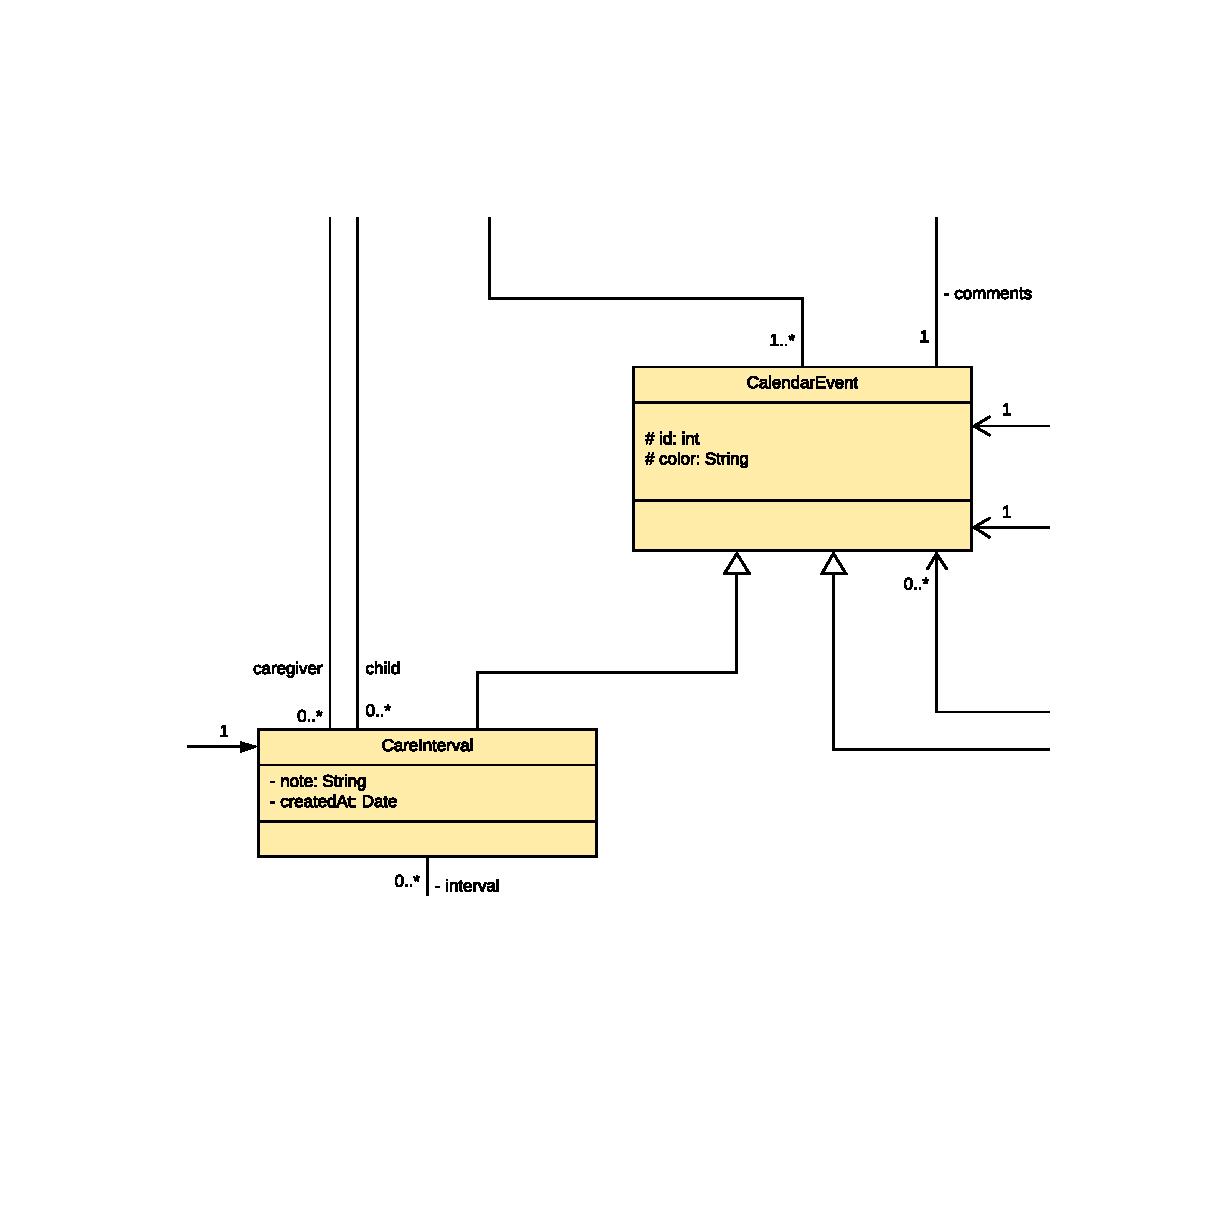
\includegraphics[width=0.7\textwidth]{pdfs/CareDays1}
	            \caption[Návrh pečovatelských dnů]{Návrh pečovatelských dnů podle Doménového modelu předmětu BI-SP2}\label{image:caredays1}
            \end{figure}
            Aktuální návrh pečovatelských dnů je příliš komplikovaně navržen\ref{imgae:caredays1}. Dlouhodobá nastavení pečovatelských dnů rodičů nevyžaduje komplikovaný návrh intervalů (viz. sekci \ref{analyza:pozadavky-frontendu}). Také je potřeba přidat odkaz na konkretního rodiče, který je zodpovědný za tento den pro zjednodušení práce s touto entitou v rámci frontedové části aplikace. Pro návrh jednorázových změn pečovatelských dnů aktuální návrh je vhodnější než pro dlouhodobá pravidla, protože komplikované intervaly jsou vyžadovány. Popis navržených změn a následné implementace bude popsán v sekci \ref{navrh:upravy:caredays}
    % \section{Analýza konkurence}
    %     Tento návrh...
% \section{Analýza testování}

\section{Analýza bezpečnosti}
    
    \subsection{Role}\label{analyza:bezpecnost:role}
    
    % Aplikace je navržená tak, že první věc, kterou uživatel udělat, je registrace. Uživatel potřebuje zvolit jméno, příjmení, email a heslo. Na základě těchto údajů se vytváří účet uživatele. V Doménovém modelu tato třída se jmenuje \textit{User}. V tento okamžik uživatel má role \textit{USER}, která mu nadává možnost udělat jenom omezený počet věcí.  
        Než se uživatel přihlásí do rodiny, nemá žádnou roli nebo má roli uživatele bez rodiny. V takovém stavu uživatel by měl mít velice omezena přístupová práva. 
        
        \begin{figure}
	        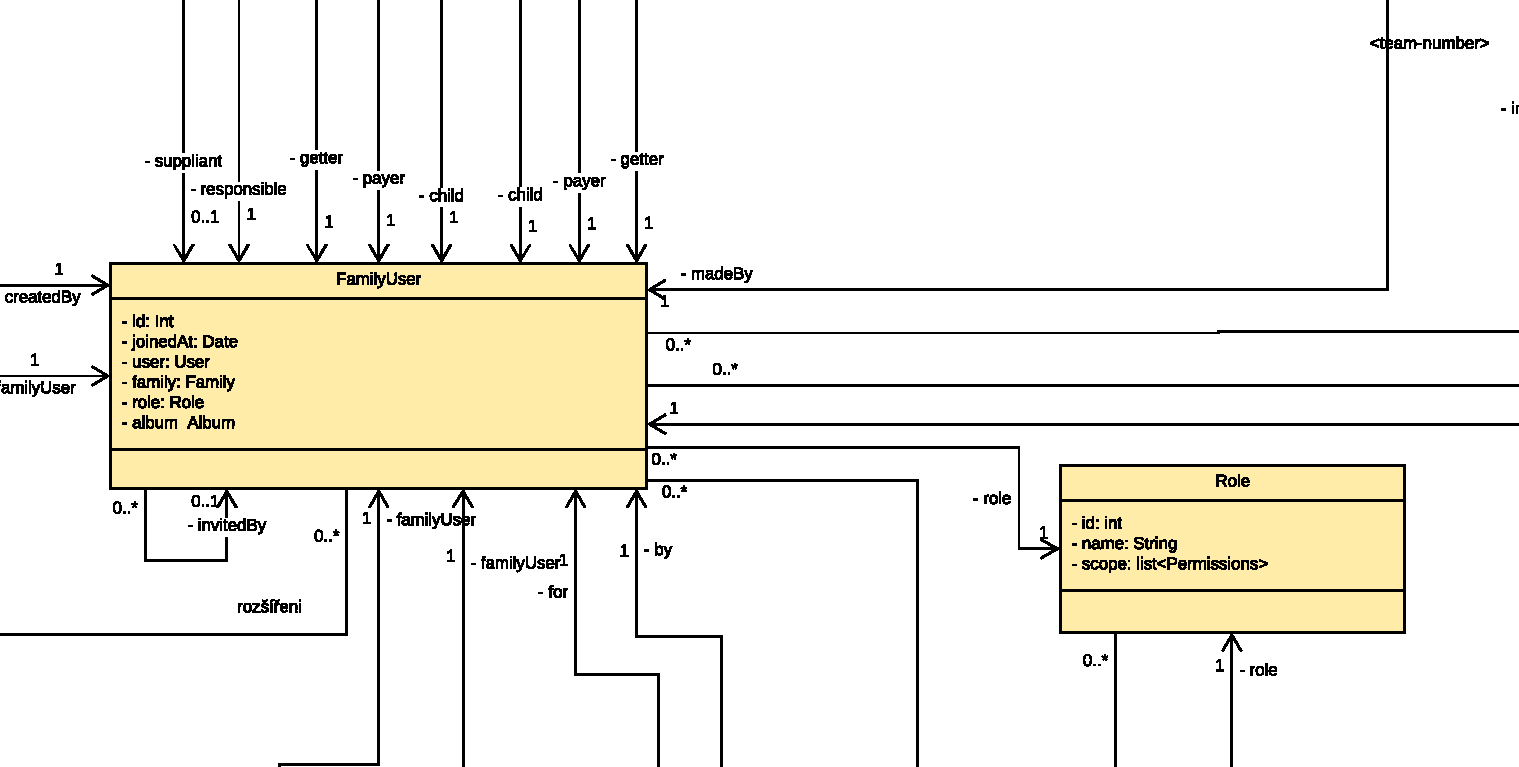
\includegraphics[width=0.7\textwidth]{pdfs/Role1}
	        \caption[Návrh \textit{Role}]{Návrh entity \textit{Role} podle Doménového modelu z předmětu BI-SP2}\label{image:Role1}
        \end{figure}
        Po přihlášeni do rodiny uživatel má svou vlastní roli (viz. obrázek \ref{image:Role1}), podle které mohou lišit jeho přístupová práva. Hlavní rolí v aplikace je rodič. Uživatel s takovou rolí má přístup ke všem potřebám dítěte a všem záznamem v kalendáři. Také, rodič může vytvořit pozvání do rodiny pro libovolného uživatele a nastavit mu libovolnou roli, včetně roli rodiče. Mimořádnou roli v rámci systému je dítěte. Uživatel s takovou rolí nemůže vlastnit pečovatelský den nebo splnit přání. Přihlášení dítěte muže proběhnout i bez vytvořeni klasického uživatele systému. Ostatní uživatele v rodině mají roli příbuzného.
    
    \subsection{Autorizace}
        Návrh bezpečné aplikace nebyl cílem předmětu zmíněných v sekcích \ref{analyza:navrh:sp1} a \ref{analyza:navrh:sp2}. Proto návrh a současná implementace neobsahuje proces přihlašovaní uživatele do systému. Nový procesu přihlašovaní bude zmíněn v sekci \ref{navrh:bezpecnost}.
        
\section{Analýza testování}\label{analyza:testovani}
    Současný návrh neobsahuje informaci o implementaci testování. Současná implementace obsahuje jednu třídu, obsahující test, který se zaměřuje na ověření, zda se načetl {kontext aplikace}\footnote{Pokročilý kontejner, který funguje podobně \textit{BeanFactory}. Načítá definice beanů, provazuje je a vydává v případe nutnosti} (viz. obrázek \ref{code:test-context-loads1}).
    \begin{figure}
    \begin{minted}{java}
@RunWith(SpringRunner::class)
@SpringBootTest
class RozvodyApplicationTests {

    @Test
    fun contextLoads() {
    }

}
        \end{minted}
        \caption{Ukázka současného testování} 
        \label{code:test-context-loads1}
        \end{figure}
\section{Průběžná integrace}
    TODO CI
   